% =============================================================================
% PESSOA 2 — SEÇÃO 3.2 (POWER ANALYSIS & FAILURE MODES)
% Padrão: ACM sigconf (\documentclass[sigconf]{acmart})
% =============================================================================

\subsection{Statistical Power Audit \& Tokenization Failure Modes}
\label{sec:power_and_failures}

Showing that downstream differences are statistically indistinguishable from zero ($p > 0.05$) does not prove equivalence unless the evaluation possesses sufficient statistical power to detect meaningful regressions. Following Miller (Section~5)~\cite{miller2024adding} and cluster-inference theory~\cite{abadie2022when}, we compute the Minimum Detectable Effect (MDE) at $80\%$ power ($1-\beta=0.80, z_{0.80}=0.842$) and two-sided $\alpha=0.05$ ($z_{0.975}=1.960$), along with the required sample size $N_{\mathrm{req}}$ to detect a target accuracy drop $\Delta$:
\begin{equation}
\mathrm{MDE} = (z_{1-\alpha/2} + z_{1-\beta})\,\mathrm{SE}_{A-B,\mathrm{clustered}}, \quad
\end{equation}
\begin{equation}
N_{\mathrm{req}}(\Delta) = \frac{2(z_{1-\alpha/2} + z_{1-\beta})^2 (1-\rho)\,p(1-p)\,\mathrm{DEFF}}{\Delta^2}.
\label{eq:mde_power}
\end{equation}

\begin{figure}[t]
    \centering
    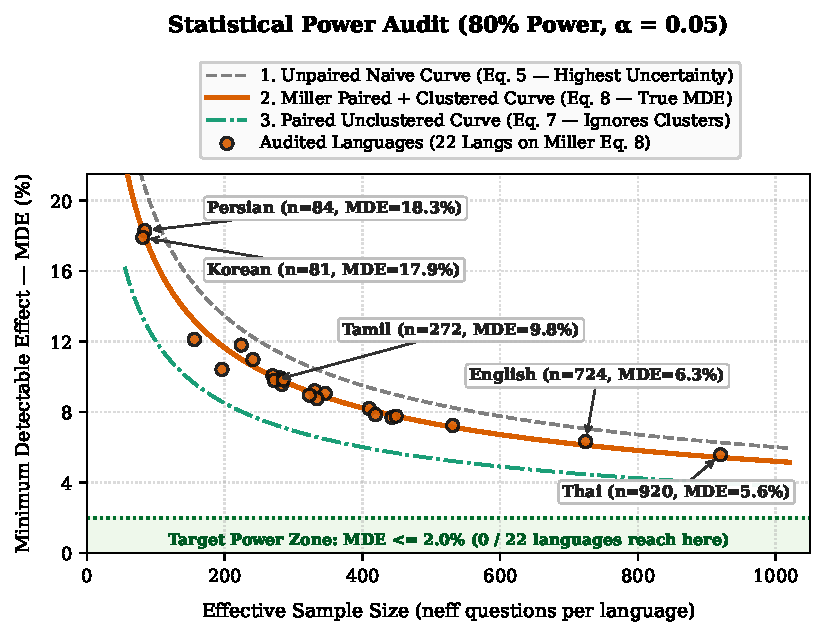
\includegraphics[width=\columnwidth]{figures/fig2_power_mde.pdf}
    \vspace{-1.5em}
    \caption{Minimum Detectable Effect (MDE) at $80\%$ power ($\alpha=0.05$) as a function of effective sample size $n_{\mathrm{eff}}$. Overlaying the 22 languages from Table~2 of~\cite{foroutan2026parity} reveals that \textbf{0 out of 22 languages} reach the adequate power zone ($\mathrm{MDE} \le 2.0\%$).}
    \label{fig:power_mde}
    \vspace{-1.0em}
\end{figure}

\textbf{Severe Under-Powering Across Languages:} Figure~\ref{fig:power_mde} demonstrates that \textbf{22 out of 22 languages ($100\%$)} are statistically underpowered to detect a $1.0\%$ or $2.0\%$ accuracy degradation. Across all 22 languages, the mean MDE is $\pm 11.38\%$ under naive unpaired errors (Eq.~5 of~\cite{miller2024adding}), drops to $\pm 7.22\%$ with question-level pairing (Eq.~7), and rebounds to $\mathbf{\pm 9.88\%}$ under Miller's paired-and-clustered estimator (Eq.~8). Even the highest-coverage languages---Thai ($n_{\mathrm{eff}} = 920, \mathrm{MDE} = \pm 5.58\%$) and English ($n_{\mathrm{eff}} = 724, \mathrm{MDE} = \pm 6.27\%$)---cannot reliably detect drops smaller than $5.5\%$. For single-benchmark languages such as Korean ($n_{\mathrm{eff}} = 81, \mathrm{MDE} = \pm 17.75\%$) and Persian ($n_{\mathrm{eff}} = 84, \mathrm{MDE} = \pm 18.29\%$), the evaluation is blind to regressions of up to 18 percentage points. In the 22-language global aggregate, cross-lingual clustering across parallel benchmarks~\cite{nllb2022no} inflates the global MDE from $\pm 1.60\%$ to $\mathbf{\pm 4.48\%}$. Consequently, actual statistical power across languages averages just $6.2\%$ for a $1.0\%$ drop and $9.7\%$ for a $2.0\%$ drop; achieving $\mathrm{MDE} \le 2.0\%$ requires an average of $N_{\mathrm{req}}=6{,}723$ clustered questions per language ($26.8\times$ the current benchmark size).

\begin{table}[t]
\centering
\caption{Algorithmic failure modes of Parity-Aware BPE (Hybrid Fair-Max)~\cite{foroutan2026parity} vs.\ Classical BPE under \texttt{Whitespace()} pre-tokenization. Phase-1 global merges preserve common tokens, whereas Phase-2 \textit{fair-max} reallocation fragments high-resource long-tail morphemes and digits.}
\vspace{-0.6em}
\footnotesize
\setlength{\tabcolsep}{2.8pt}
\begin{tabular}{lcccc}
\toprule
\textbf{Domain / Failure Mode} & \textbf{Classical} & \textbf{PA-Hybrid} & \textbf{Ratio} & \textbf{Overhead} \\
\midrule
Code Syntax (Python)       & 16 & 26 & 1.62 & $+62.5\%$  \\
Mathematical / Numeric     & 19 & 37 & 1.95 & $+94.7\%$  \\
Structured JSON / API      & 23 & 52 & 2.26 & $+126.1\%$ \\
German Compound Nouns      & 12 & 35 & 2.92 & $+191.7\%$ \\
English STEM Terminology   & 10 & 43 & 4.30 & $+330.0\%$ \\
\bottomrule
\end{tabular}
\vspace{-0.8em}
\label{tab:failure_modes}
\end{table}

\textbf{Tokenization Failure Modes in Specialized Domains:} To understand where PA-BPE's compression loss manifests structurally, we execute both Classical BPE and Hybrid PA-BPE (\textit{fair-max}, Eq.~6 of~\cite{foroutan2026parity}) with the official \texttt{Whitespace()} pre-tokenizer across five technical domains (Table~\ref{tab:failure_modes}). While Phase-1 global merges preserve top-frequency keywords (\texttt{def}, \texttt{return}, \texttt{and}, \texttt{und}), Phase-2 reallocates tail merges toward low-resource scripts (Tamil, Telugu, Korean, Persian), inducing severe over-segmentation in structured inputs:
\begin{itemize}
    \item \textbf{Code \& Structured JSON ($+62.5\%$ to $+126.1\%$ overhead):} Domain identifiers (\texttt{calculate} $\rightarrow$ \texttt{c|al|c|ul|at|e}) and JSON schema keys/enums (\texttt{transaction}, \texttt{PENDING\_VERIFICATION}) shatter into character fragments, inflating KV-cache memory and structured decoding latency~\cite{petrov2023language,ahia2023all}.
    \item \textbf{Numbers \& Arithmetic (1.95 tokens):} Classical BPE consolidates recurring 3-digit blocks (\texttt{141|592|653}), whereas PA-BPE fragments decimal mantissas into single and paired digits (\texttt{1|4|1|59|2...}), impairing positional alignment in multi-digit arithmetic~\cite{singh2024tokenization}.
    \item \textbf{German Compounds \& STEM (2.92 to 4.30 tokens):} Productive German compound roots (\texttt{schiff|fahrts} $\rightarrow$ \texttt{sch|if|f|f|a|h|r|ts}) and Latin/Greek STEM morphemes (\texttt{neuro|degenerative} $\rightarrow$ 12 sub-tokens) lose morphological coherence, explaining localized NLU variance~\cite{foroutan2026parity}.
\end{itemize}
